\chapter{\ac{ARG} Testing}
\label{chp:testseq}
\par This appendix covers the steps used to run a test. The events shown below occur in order for each test. 

\begin{comment}
\section{Network Setup}
\par As Section \ref{sec:evaluation_technique} discusses, tests are run on a seven-node network, laid out as illustrated in Figure \ref{fig:argnetwork_app}.
\begin{figure}
	\centering
	\caption{ARG Network Layout Overview}
	\label{fig:argnetwork_app}
	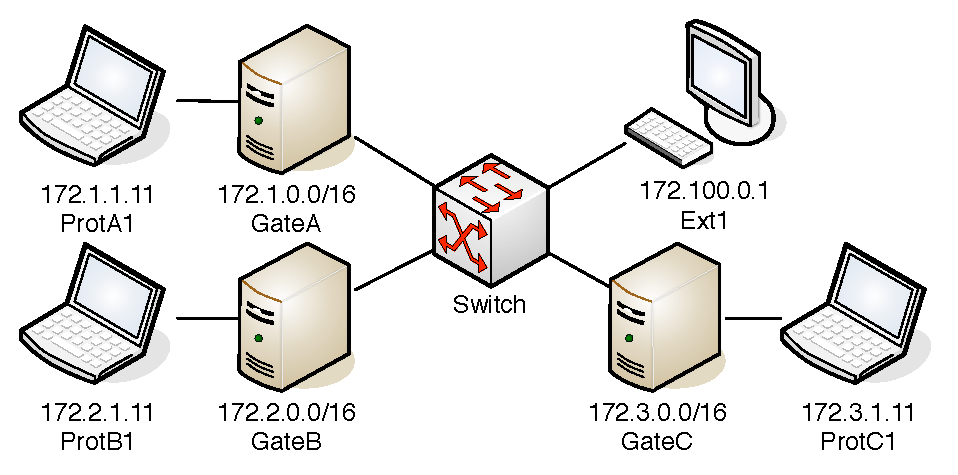
\includegraphics[width=0.75\textwidth]{thesis_network}
\end{figure}

\section{Test Sequence}
\end{comment}

\begin{enumerate}
\item Set time on all hosts to be the as similar as possible (used for post-processing only).
\item Set artificial network latency on external interfaces of gates.
\item Start \texttt{tcpdump} on each host. Gateways have two instances started, one for each interface. The exact commands with the appropriate traffic filters appear in Table \ref{tbl:test_tcpdump_calls}.
\begin{table}
\caption{Test run \texttt{tcpdump} calls}
\label{tbl:test_tcpdump_calls}
\centering
\begin{tabular}{l|l}
Host & Command\\
\hline
Gateway & \texttt{sudo tcpdump -i eth2 -w gateX-inner.pcap -n ip and not arp}\\
	& \texttt{sudo tcpdump -i eth1 -w gateX-outer.pcap -n ip and not arp}\\
\hline
Prot/Ext & \texttt{sudo tcpdump -i eth1 -w clientX.pcap -n ip and not arp}
\end{tabular}
\end{table}

\item Set \ac{ARP} cache size on gateways and external host to allow for 65,536 entries. This is needed at high hop rates only because all systems are on the same network segment.
\item Push configuration files for \ac{ARG}. \texttt{ProtA1} and \texttt{ProtC1} each know about \texttt{ProtB1}, but not about each other. \texttt{ProtB1} is given configuration files for both \texttt{ProtA1} and \texttt{ProtC1}.
\item Start \ac{ARG} on the gateways. 
\item Start traffic generators on hosts, as appropriate for the test being run. See Section \ref{sec:exp_design} for general flow of traffic for each test type.
\item Wait for the test to finish. For all tests discussed in this thesis, tests run for five minutes.
\item Stop traffic generators.
\item Stop \ac{ARG}.
\item Stop traffic collectors (\texttt{tcpdump}).
\item Retrieve log and pcap files from every host into a directory.
\end{enumerate}

\par After the logs are collected together, the run is processed by a separate script, \texttt{process\_run.py}. See Appendix \ref{chp:processor} for details on its use. 

